% =====================================================================
% COMP8240 Applications of Data Science -- Assessment 3: Project Final Report
% Novel project: replication of Shi et al. (ICLR 2024), Min-K% Prob.
% Numbers come from generated/numbers.tex (scripts/make_report_assets.py); do not type results by hand.
% Build:  latexmk -pdf main.tex
% =====================================================================
\documentclass[11pt]{article}
\usepackage[preprint]{acl}

\usepackage{times}
\usepackage{latexsym}
\usepackage[T1]{fontenc}
\usepackage[utf8]{inputenc}
\usepackage{microtype}
\usepackage{graphicx}
\usepackage{booktabs}
\usepackage{amsmath}
\usepackage{array}
\usepackage{xcolor}

\newcommand{\pending}{\textcolor{red}{[pending]}}
\newcommand{\TODO}[1]{\textcolor{red}{[TODO: #1]}}
\newcolumntype{L}[1]{>{\raggedright\arraybackslash}p{#1}}
% Generated by scripts/make_report_assets.py from results/ -- do not edit by hand.
\newcommand{\RepPPL}{0.626}
\newcommand{\NewPPL}{0.661}
\newcommand{\RepZlib}{0.642}
\newcommand{\NewZlib}{0.627}
\newcommand{\RepLower}{0.603}
\newcommand{\NewLower}{0.642}
\newcommand{\RepRef}{0.610}
\newcommand{\NewRef}{0.611}
\newcommand{\RepMinK}{0.649}
\newcommand{\NewMinK}{0.675}
\newcommand{\RepMinKTPR}{14.6}
\newcommand{\RepZlibTPR}{17.1}
\newcommand{\RepSizeTrend}{0.558, 0.591, 0.617, 0.618, 0.649}
\newcommand{\RepMinKShort}{0.617}
\newcommand{\RepMinKLong}{0.701}
\newcommand{\RepCIShort}{0.58--0.66}
\newcommand{\RepCILong}{0.57--0.81}
\newcommand{\RepBestK}{20\%}
\newcommand{\RepMarginZlib}{0.007}
\newcommand{\NewSizeTrend}{0.561, 0.641, 0.675}
\newcommand{\BlindWikiRaw}{0.955}
\newcommand{\BlindWikiNoyr}{0.789}
\newcommand{\BlindWikiYear}{0.889}
\newcommand{\BlindNewRaw}{0.947}
\newcommand{\BlindNewNoyr}{0.797}
\newcommand{\BlindNewYear}{0.889}
\newcommand{\BlindArxRaw}{0.952}
\newcommand{\BlindArxNoyr}{0.940}
\newcommand{\BlindArxYear}{0.623}
\newcommand{\BlindMimirRaw}{0.519}
\newcommand{\BlindMimirNoyr}{0.524}
\newcommand{\BlindMimirYear}{0.491}
\newcommand{\BlindArxLeaky}{0.997}
\newcommand{\BlindMimirRange}{0.48--0.55}
\newcommand{\MimirPPL}{0.525}
\newcommand{\MaskWikiPPL}{0.592}
\newcommand{\MaskNewPPL}{0.628}
\newcommand{\MimirZlib}{0.528}
\newcommand{\MaskWikiZlib}{0.611}
\newcommand{\MaskNewZlib}{0.586}
\newcommand{\MimirLower}{0.511}
\newcommand{\MaskWikiLower}{0.571}
\newcommand{\MaskNewLower}{0.633}
\newcommand{\MimirRef}{0.514}
\newcommand{\MaskWikiRef}{0.602}
\newcommand{\MaskNewRef}{0.601}
\newcommand{\MimirMinK}{0.529}
\newcommand{\MaskWikiMinK}{0.610}
\newcommand{\MaskNewMinK}{0.628}
\newcommand{\MimirSizeTrend}{0.512, 0.522, 0.529}
\newcommand{\MimirCI}{0.50--0.56}
\newcommand{\MaskWikiDrop}{0.039}
\newcommand{\MaskNewDrop}{0.047}
\newcommand{\MaskShareRange}{26--27\%}
\newcommand{\RepSizeGain}{0.091}
\newcommand{\NewSizeGain}{0.114}
\newcommand{\MimirSizeGain}{0.017}
\newcommand{\JudgeQwenWiki}{0.705}
\newcommand{\JudgeQwenNew}{0.667}
\newcommand{\JudgeQwenMimir}{0.489}
\newcommand{\JudgeQwenPairAcc}{0.53}
\newcommand{\JudgeQwenOrderAcc}{0.48/0.52}
\newcommand{\JudgeQwenConsistent}{0.00}
\newcommand{\JudgeQwenPA}{0.00}
\newcommand{\JudgeQwenMass}{1.00}
\newcommand{\JudgePhiWiki}{0.733}
\newcommand{\JudgePhiNew}{0.643}
\newcommand{\JudgePhiMimir}{0.507}
\newcommand{\JudgePhiPairAcc}{0.64}
\newcommand{\JudgePhiOrderAcc}{0.47/0.53}
\newcommand{\JudgePhiConsistent}{0.02}
\newcommand{\JudgePhiPA}{0.01}
\newcommand{\JudgePhiMass}{1.00}
\newcommand{\ShiftMinKRange}{0.53--0.76}
\newcommand{\ShiftBlindRange}{0.50--0.62}
\newcommand{\ShiftMinKPooled}{0.64}
\newcommand{\ShiftNMin}{26}
\newcommand{\ShiftNMax}{194}
\newcommand{\FleissKOne}{0.005}
\newcommand{\CohenHumanRangeOne}{$-$0.06 to 0.04}
\newcommand{\MajorityAccOne}{0.54}
\newcommand{\HumanAccRangeOne}{0.47--0.64}
\newcommand{\HumanMedianRangeOne}{1.5--4.1}
\newcommand{\HumanTotalRangeOne}{4--17}
\newcommand{\KappaQwenMajorityOne}{0.25}
\newcommand{\JudgeQwenPairAccOne}{0.53}
\newcommand{\KappaPhiMajorityOne}{0.21}
\newcommand{\JudgePhiPairAccOne}{0.64}
\newcommand{\KappaJudgesOne}{0.41}
\newcommand{\PairMinKOne}{0.64}
\newcommand{\PairBlindOne}{0.97}
\newcommand{\PairBlindNoyrOne}{0.83}
\newcommand{\KappaMinKMajorityOne}{0.04}
\newcommand{\FleissKTwo}{0.100}
\newcommand{\CohenHumanRangeTwo}{$-$0.02 to 0.24}
\newcommand{\MajorityAccTwo}{0.62}
\newcommand{\HumanAccRangeTwo}{0.47--0.68}
\newcommand{\HumanMedianRangeTwo}{12.9--21.1}
\newcommand{\HumanTotalRangeTwo}{11--25}
\newcommand{\KappaQwenMajorityTwo}{0.34}
\newcommand{\JudgeQwenPairAccTwo}{0.50}
\newcommand{\KappaPhiMajorityTwo}{0.34}
\newcommand{\JudgePhiPairAccTwo}{0.65}
\newcommand{\KappaJudgesTwo}{0.38}
\newcommand{\PairMinKTwo}{0.68}
\newcommand{\PairBlindTwo}{0.95}
\newcommand{\PairBlindNoyrTwo}{0.80}
\newcommand{\KappaMinKMajorityTwo}{0.19}
\newcommand{\SnipWikiMember}{Hurricane Ana was the second tropical cyclone in 2014 to threaten the U.S. state of Hawaii with a direct hit, after Iselle in August. The twenty-first named storm and fifteenth hurricane of}
\newcommand{\SnipWikiNon}{The 12th Circle Chart Music Awards ceremony was held at KSPO Dome in Seoul on February 18, 2023, to recognise the best artists and recordings, primarily based on Circle Music Chart of}
\newcommand{\SnipNewMember}{The United Central Luzon Athletic Association (UCLAA) is an association of colleges and universities in Central Luzon region aiming to showcase the skills of student-athletes in different sports. It was formally introduced}
\newcommand{\SnipNewNon}{Question 3 is a voter referendum that will be held on November 3, 2026. If approved by voters, it would exempt Maryland's congressional districts from guidelines in the Constitution of Maryland that}
\newcommand{\SnipNewJSON}{\{"input": "Question 3 is a voter referendum that ...", "label": 0, "title": "2026 Maryland Question 3", "created": "2026-08-04T22:58:17Z", "pageid": 83869129, "revid": 1379019453\}}

\setlength{\emergencystretch}{3em}   % fewer overfull lines from long \texttt names

\title{Detecting Pretraining Data, or Detecting the Passage of Time?\\
A Replication of Min-K\% Prob on WikiMIA and New Data}

\author{Ashikur Rahman \\
  Student ID: 48483818 \quad
  COMP8240, Session 2 2026 \\
  School of Computing, Macquarie University \\
  \texttt{ashikur.rahman1@students.mq.edu.au}}

\begin{document}
\maketitle

\begin{abstract}
I replicate \emph{Detecting Pretraining Data from Large Language Models} \citep{shi2024detecting}, which proposes Min-K\% Prob, a reference-free test of whether a passage was in a model's training data, and the WikiMIA benchmark. With the authors' unmodified code and five Pythia models (160M--2.8B), every method's mean AUC lands within about 0.02 of the paper's Pythia-2.8B results (Min-K\% \RepMinK{} against 0.67), and size and length trends reproduce. I then build WikiMIA-2026, a 2,078-passage re-run of the paper's recipe with a 2026 cut-off, a shift-controlled subset of it and a 100-pair human annotation set, and add two existing benchmarks. Min-K\% transfers to the new data (AUC \NewMinK{}), but a text classifier that never sees the model separates the same passages with AUC \BlindNewRaw{}. On MIMIR, where both classes come from the same period, Min-K\% scores \MimirMinK{}, close to chance, and its size trend almost vanishes. Masking years removes only \MaskShareRange{} of its margin over chance, and two small LLM judges that only read the masked text beat it on WikiMIA, come within 0.04 on WikiMIA-2026 and fall to chance on MIMIR. The results are consistent with substantial temporal confounding: a WikiMIA-style AUC alone cannot show that an attack detects membership.
\end{abstract}

% =====================================================================
\section{Introduction}

Language-model developers rarely publish their training corpora, yet authors, benchmark designers and data subjects all have reasons to ask whether a particular text was used. \emph{Membership inference}---deciding from model outputs whether a text was in the training set \citep{shokri2017membership}---is the technical question underneath. \citet{shi2024detecting} brought it to LLM pretraining with a simple statistic and a dynamic benchmark, and both have since become standard reference points.

The project has three parts. I \emph{reproduce} the paper's WikiMIA results with the original code (Section~\ref{sec:replication}); I \emph{apply} it to data the authors never used: MIMIR, three datasets I built, and arXivTection for a model-free audit (Section~\ref{sec:newdata}); and I \emph{test} the paper's central claim against a known objection, that date-defined benchmarks reward detecting \emph{when} a text was written rather than \emph{whether} it was trained on \citep{duan2024membership,das2024blind} (Section~\ref{sec:results}). All code, distributable data, per-passage scores and logs are public.\footnote{\url{https://github.com/Ashik-here/COMP8240-MinK-Replication}} Along the way the project uses most of the unit's toolkit: cloud virtual machines (Colab GPUs for model runs, a GitHub Codespaces configuration for the CPU scripts), git, \LaTeX{} with BibTeX, Wikipedia data gathering through the MediaWiki API with regular-expression cleaning, analysis in pandas and scikit-learn, human annotation with Cohen's and Fleiss' $\kappa$, and an LLM-as-judge checked against the annotators.

% =====================================================================
\section{The Paper, and Why I Chose It}
\label{sec:paper}

\paragraph{Summary.} \citet{shi2024detecting}\footnote{\url{https://openreview.net/forum?id=zWqr3MQuNs}} ask whether an outsider with only query access to a model can tell that a passage was in its pretraining data. Their method, \textbf{Min-K\% Prob}, rests on one observation: an unseen passage tends to contain a few tokens the model finds very unlikely, and training removes such outliers. For $x=x_1\ldots x_N$, let $\mathrm{Min\text{-}K\%}(x)$ be the $k\%$ of tokens with the lowest probability under the model; the score is
\begin{equation}
\frac{1}{|\mathrm{Min\text{-}K\%}(x)|}\sum_{x_i\in\mathrm{Min\text{-}K\%}(x)}\log p(x_i\mid x_{<i}),
\end{equation}
with higher scores predicting membership. It needs no reference model and one forward pass per passage. The paper also introduces \textbf{WikiMIA} (Section~\ref{sec:wikimia}) and three case studies: copyrighted books, contaminated benchmarks, and auditing machine unlearning.

\paragraph{Evaluation framework.} Detection is scored as binary classification with members as positives, using two threshold-free measures: \textbf{AUC}, the probability that a random member outscores a random non-member, and \textbf{TPR at 5\% FPR}, the share of members caught when only 5\% of non-members are falsely flagged, which matters when an accusation must be made about a specific document \citep{carlini2022membership}. Baselines are perplexity (\textsc{PPL}; \citealp{yeom2018privacy}), \textsc{Zlib} and \textsc{Lowercase} calibration \citep{carlini2021extracting}, a smaller reference model (\textsc{Smaller Ref}) and the costly \textsc{Neighbor} attack \citep{mattern2023membership}. Averaged over five models and the original and paraphrased versions of WikiMIA, Min-K\% reaches an AUC of 0.72 against 0.67 for the best baseline, PPL: the paper's headline 7.4\% improvement. On the original version with Pythia-2.8B, the model this project centres on, the paper reports Min-K\% 0.67, Zlib 0.65, PPL 0.61, Smaller Ref 0.60 and Lowercase 0.59.

\paragraph{Justification.} \emph{Venue:} ICLR is ranked A* by CORE (CORE2023, FoR 4611; \citealp{core2023}) and is the 8th-ranked venue across all disciplines in Google Scholar Metrics 2025, with h5-index 362 \citep{scholarmetrics2025}. \emph{Standing:} the paper has 869 citations on Google Scholar (9 November 2026); WikiMIA is the standard evaluation set of later work at strong venues, including Min-K\%++, an ICLR 2025 Spotlight \citep{zhang2025minkpp}, and an EMNLP 2024 paper \citep{zhang2024pretraining}; and the central claim has been publicly contested \citep{duan2024membership,das2024blind}. \emph{Feasibility:} the code is public under Apache-2.0 and about 250 lines \citep{minkcode2023}; the data is 469\,KB under an MIT licence; and the Pythia models \citep{biderman2023pythia} run on a free Colab T4. Pythia also has a public, documented training corpus, the Pile \citep{gao2020pile}, which is what makes a membership ground truth that does not depend on dates possible (Section~\ref{sec:existing}).

% =====================================================================
\section{The Original Datasets}
\label{sec:wikimia}

WikiMIA\footnote{\url{https://huggingface.co/datasets/swj0419/WikiMIA}} \citep{wikimia2023} defines membership by time. Wikipedia event pages created after 1 January 2023 cannot have been in the training data of models released before then and are labelled non-members (0); pages about events created before 2017 almost certainly were and are labelled members (1). The passages are the opening words of each article, cut to 32, 64, 128 or 256 words, giving four splits of 776, 542, 250 and 82 passages (387, 284, 139 and 51 members). Each split is a list of records with two fields, \texttt{input} and \texttt{label}, which the original code reads directly; there is no title, date or page identifier. Figure~\ref{fig:snippets} shows one member and one non-member. The splits shrink with length because only long articles reach 256 words, so the four splits are not independent samples.

\paragraph{Other data in the paper.} WikiMIA also has a \emph{paraphrased} version, each passage rewritten by ChatGPT, which tests whether a detector depends on exact wording; the paper reports both versions, and I replicate the original. The case studies use data of their own. \emph{BookMIA} holds 512-word snippets, 100 per book, from 50 books ChatGPT has memorised \citep{chang2023speak} and 50 first published in 2023; it sets a threshold then applied to 100 books from the Pile's Books3. The contamination study inserts 200 examples from each of BoolQ, IMDB, TruthfulQA and CommonsenseQA into RedPajama text, continues pretraining LLaMA-7B on it, and keeps 200 more of each as non-members. The unlearning audit probes LLaMA2-7B-WhoIsHarryPotter \citep{eldan2023harrypotter} with 512-word chunks of the first four Harry Potter books and 1,000 GPT-4-written questions.

\begin{figure*}[t]
\centering\footnotesize
\begin{tabular}{@{}L{2.2cm}L{1.9cm}L{10.9cm}@{}}
\toprule
\textbf{Dataset} & \textbf{Label} & \textbf{\texttt{input} (32-word split)} \\
\midrule
WikiMIA & 1 (member) & \SnipWikiMember \\
WikiMIA & 0 (non-member) & \SnipWikiNon \\
\addlinespace
WikiMIA-2026 & 1 (member) & \SnipNewMember \\
WikiMIA-2026 & 0 (non-member) & \SnipNewNon \\
\midrule
\multicolumn{3}{@{}L{15.4cm}@{}}{\textbf{One WikiMIA-2026 record} (passage shortened here): {\ttfamily\footnotesize \SnipNewJSON}} \\
\bottomrule
\end{tabular}
\caption{Data snippets. WikiMIA records hold only \texttt{input} and \texttt{label}; WikiMIA-2026 keeps the same two fields, so the original code reads it unchanged, and adds the title, creation timestamp, page id and the exact revision the text was taken from. Note the date and the future tense in the non-member passages: Section~\ref{sec:results} measures how much of the benchmark these cues explain.}
\label{fig:snippets}
\end{figure*}

% =====================================================================
\section{Replication of the Original Work}
\label{sec:replication}

\paragraph{Environment.} All model runs used Google Colab with one NVIDIA T4 (16\,GB), Python 3.13, CUDA 13, \texttt{datasets} 4.8 and \texttt{scikit-learn} 1.6, with PyTorch 2.11 and \texttt{transformers} 5.18 for the replication and WikiMIA-2026 (2.14 and 5.22 for the later controls, after a Colab update), all recorded in \texttt{results/*/environment.json}. The original repository is cloned and checked out at commit \texttt{a5048f9}; its files are never edited. The notebooks import \texttt{run.py} and call its own functions (\texttt{load\_model}, \texttt{evaluate\_data}, \texttt{sweep}), so scoring and evaluation are the authors' code, while the per-passage scores that \texttt{run.py} discards are saved. I added 1,000-sample bootstrap 95\% confidence intervals on every AUC \citep{efron1993introduction}, which the paper does not report. Targets are Pythia 160M, 410M, 1B, 1.4B and 2.8B with Pythia-70M as the \textsc{Smaller Ref} model, the reference the paper uses for Pythia-2.8B, on all four WikiMIA lengths. Under \texttt{transformers}~5 the loader keeps the checkpoints' float16 weights. A full sweep takes about 35 minutes.

\paragraph{Six traps.} Getting a correct number required finding six traps in the code, listed in Appendix~\ref{app:traps} and the repository README. The worst: \texttt{run.py} negates the Min-K\% score and \texttt{eval.py} negates it again, so a reimplementation that misses one sign inverts the ROC curve; and the GPT-3 path calls a model retired in January 2024.

\begin{table*}[t]
\centering\footnotesize
\begin{tabular}{@{}lccccc>{\bfseries}cc@{}}
\toprule
 & \multicolumn{5}{c}{\textbf{AUC (mine)}} & & \textbf{TPR@5\%} \\
\cmidrule(lr){2-6}
\textbf{Method} & 32 & 64 & 128 & 256 & mean & \textbf{paper} & mine / paper \\
\midrule
PPL & 0.614 & 0.584 & 0.629 & 0.678 & 0.626 & 0.61 & 9.6 / 9.4 \\
Zlib & 0.621 & 0.605 & 0.650 & 0.693 & 0.642 & 0.65 & 17.1 / 18.7 \\
Lowercase & 0.609 & 0.577 & 0.595 & 0.629 & 0.603 & 0.59 & 8.4 / 10.8 \\
Smaller Ref & 0.611 & 0.597 & 0.599 & 0.634 & 0.610 & 0.60 & 7.7 / 10.1 \\
\textbf{Min-K\% (k=20)} & \textbf{0.617} & \textbf{0.612} & \textbf{0.669} & \textbf{0.701} & \textbf{0.649} & 0.67 & 14.6 / 13.7 \\
\bottomrule
\end{tabular}

\caption{Replication on WikiMIA with Pythia-2.8B and the original code. AUC per passage length and the mean of the four, against the paper's Table~1 (original version), which does not say which length it reports; TPR at 5\% FPR (\%, mean of the four lengths) against the paper's Table~6. Every mean AUC is within about 0.02 of the paper. 95\% bootstrap CIs are about $\pm$0.04 at 32 words and $\pm$0.12 at 256 words (\texttt{results/replication/summary.csv}).}
\label{tab:replication}
\end{table*}

\paragraph{Results.} Table~\ref{tab:replication} compares Pythia-2.8B with the paper. Every method's mean AUC is within about 0.02 of the published value, and the ordering of the methods matches the paper's: Min-K\% first (\RepMinK{} vs 0.67), then Zlib, PPL, Smaller Ref and Lowercase. Both trends the paper reports also reproduce (Figure~\ref{fig:size}): Min-K\% improves monotonically with model size (\RepSizeTrend{} from 160M to 2.8B) and, apart from a dip at 64 words, with passage length (\RepMinKShort{} at 32 words to \RepMinKLong{} at 256). In a sweep of $k$ from 5\% to 60\%, $k$=\RepBestK{}, the paper's recommended value, is the best on average.

\begin{figure}[t]
\centering
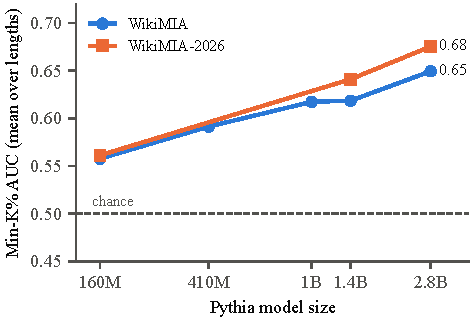
\includegraphics[width=\columnwidth]{figures/size_trend.pdf}
\caption{Min-K\% AUC against Pythia size on the original WikiMIA (five sizes) and on the new data. Mean over lengths; dashed line is chance. The upward trend the paper reports reproduces on both WikiMIA and WikiMIA-2026.}
\label{fig:size}
\end{figure}

\paragraph{How close, and why not closer.} The replication succeeds on its own terms, but two qualifications matter. First, Min-K\%'s margin over Zlib is \RepMarginZlib{} AUC, and a paired bootstrap over the same passages (\texttt{scripts/paired\_bootstrap.py}) puts the difference between $-$0.020 and 0.034 (95\%): at this scale the data cannot separate Min-K\% from Zlib, and by TPR at 5\% FPR Zlib is ahead (\RepZlibTPR\% vs \RepMinKTPR\%). The paper reports single numbers without intervals, so its ranking of methods is less certain than it appears. Second, the remaining differences have identifiable causes: the paper does not state which length its Table~1 uses, so I report all four and their mean; current libraries load the models in float16 rather than the float32 that 2023 versions defaulted to; and the 5\% FPR threshold is set by only the top 1--19 non-members of each split, so TPR moves by whole percentage points when a single passage changes rank.

\paragraph{Scope.} I reproduced the Pythia rows of the original version only. GPT-3 cannot be run (trap 2, Appendix~\ref{app:traps}); models of 20B--66B parameters do not fit a T4; \textsc{Neighbor} is not in the released code; and I did not get to OPT or 8-bit 7B models, which the proposal planned, or to the paraphrased version, choosing to spend the time on new data instead. One family at five sizes still tests the size claim within a single training corpus. The three case studies were scoped out in the proposal for compute and API reasons.

% =====================================================================
\section{Construction of New Data}
\label{sec:newdata}

Table~\ref{tab:datasets} summarises every dataset in the project. All are converted into the \texttt{input}/\texttt{label} schema the original code reads.

\begin{table*}[t]
\centering\footnotesize
\begin{tabular}{@{}L{2.5cm}L{4.4cm}L{4.0cm}rL{2.0cm}@{}}
\toprule
\textbf{Dataset} & \textbf{Members (1)} & \textbf{Non-members (0)} & \textbf{Passages} & \textbf{Access} \\
\midrule
WikiMIA (original) & Wikipedia events, created before 2017 & created after 1 Jan 2023 & 1,650 & HF Hub, MIT \\
\addlinespace
MIMIR Wikipedia & Pile \emph{train} split & Pile \emph{test} split, same period & 6,000 & HF Hub, gated \\
arXivTection & arXiv excerpts, papers before 2022 & papers from 2023 & 1,549 & HF Hub, MIT \\
\addlinespace
\textbf{WikiMIA-2026} (new) & event pages from 2012--15 categories, created before 2017 & event pages from 2026 categories, created in 2026 & 2,078 & this repo, CC BY-SA \\
\textbf{WikiMIA-2026-matched} (new) & \multicolumn{2}{L{8.3cm}}{subset of WikiMIA-2026 matched so a text-only classifier cannot separate the classes} & 416 & this repo, CC BY-SA \\
\textbf{Annotation set} (new) & \multicolumn{2}{L{8.3cm}}{100 member/non-member pairs from WikiMIA-2026 (64 words), years masked, labelled by 3 humans and 2 LLM judges} & 200 & this repo \\
\bottomrule
\end{tabular}
\caption{Datasets. Passage counts sum over length splits (WikiMIA and WikiMIA-2026: 32/64/128/256 words; MIMIR: 2,000 passages at each of 32/64/128). Classes are balanced in every new dataset.}
\label{tab:datasets}
\end{table*}

\subsection{Existing datasets}
\label{sec:existing}

\paragraph{MIMIR} \citep{duan2024membership,mimirdata} was built to test the objection this project examines. Its members come from the Pile's training split and its non-members from the Pile's test split, so both sides share a source and a time period; for Pythia, which was trained on exactly that training split, membership is true by construction rather than inferred from dates. I use the Wikipedia domain, which matches WikiMIA's genre, at the \texttt{ngram\_13\_0.8} threshold (1,000 members, 1,000 non-members) and cut each passage to its first 32, 64 and 128 words, the WikiMIA lengths every passage reaches. It plays the role of the shift-controlled split ND-2 in my proposal, which planned to check passages against the Pile directly; the Pile is no longer distributed by its original host, and MIMIR already implements that design.

\paragraph{arXivTection} \citep{duarte2024decop} holds 1,549 excerpts from arXiv papers, labelled by publication before 2022 or in 2023. It ships in DE-COP's multiple-choice format, one verbatim excerpt and three paraphrases per row, so an adapter keeps only the verbatim excerpt. I use it only for the blind audit (Section~\ref{sec:blind}): its dates do not match Pythia, whose Pile snapshot predates 2021, so many of its ``members'' are not Pythia members and Min-K\% on Pythia would be scored against wrong labels.

\paragraph{Not used.} BookTection has arXivTection's label mismatch; PatentMIA needs a Chinese model; the Pile held-out splits survive only on an undocumented mirror.

\subsection{WikiMIA-2026}
\label{sec:wikimia2026}

The paper calls WikiMIA a dynamic benchmark that can be refreshed as models are released, so the most faithful new dataset re-runs its recipe with a later cut-off. \texttt{scripts/build\_wikimia2026.py} does this in five steps, using a single-threaded, rate-limited MediaWiki API client that identifies itself by the repository URL (3,110 API calls in all).
(1)~\emph{Candidates.} For 16 event categories (disasters, crimes, competitions, festivals, awards, politics, science, sports, technology, transport, health and others) it lists pages under \texttt{Category:2026~<topic>} as non-member candidates and under \texttt{Category:2012}--\texttt{2015~<topic>} as member candidates, two levels deep, dropping lists, timelines and disambiguation pages.
(2)~\emph{Creation date} is the timestamp of the page's first revision. A non-member must be created on or after 1 January 2026, after the training cut-off of every model used here; a member must be created before 1 January 2017, the rule the paper uses. Of 947 non-member and 795 member candidates checked, 347 and 195 were created on the wrong side of their date and rejected.
(3)~\emph{Text} is the article's lead section, cleaned with regular expressions (reference markers, empty brackets, whitespace).
(4)~\emph{Redirects} are followed before the date check, the title filters are applied again to the resolved title, and pages reached twice are kept once. A first build applied the filters too early; I fixed this and re-made the splits from the saved candidates, which \texttt{stats.json} records.
(5)~\emph{Splits.} Passages are cut to the first 32, 64, 128 and 256 words and balanced by down-sampling members, giving 1,052, 686, 268 and 72 passages (half members). The proposal's Australian-events variant was dropped for time.

Two choices differ from WikiMIA deliberately. Both sides come from the \emph{same} category types, which WikiMIA does not document, to reduce topic differences between the classes. And every record stores its title, creation timestamp, page id and revision id (Figure~\ref{fig:snippets}), so the exact text can be recovered from Wikipedia even though pages keep changing. Two weaknesses remain. Member text is the \emph{current} revision, as in WikiMIA, so it may differ from what the model saw. And creation date is an imperfect label: a page created in 2026 by splitting an older article (for example ``Legault ministry'', covering 2018--2026) is a non-member by rule while its text may be old.

\subsection{WikiMIA-2026-matched: a shift-controlled subset}
\label{sec:matched}

The second new dataset removes, as far as the text allows, the cues that let one tell a 2026 page from a 2014 page without the model. The blind classifier of Section~\ref{sec:blind} gives each passage an out-of-fold probability of being a member, a propensity score for the time shift \citep{rosenbaum1983central}. \texttt{scripts/shift\_controlled.py} matches each member to the nearest non-member on the logit of that score, without replacement and within a caliper of 0.2 standard deviations \citep{austin2011optimal}, and keeps only matched pairs: 194, 126, 70 and 26 passages at the four lengths (100, 64, 50 and 36 when applied to WikiMIA), on which the blind classifier scores \ShiftBlindRange{} AUC, close to chance by construction. The subset is small, and it only removes cues a bag-of-words model can learn.

\subsection{Human annotation of recency}
\label{sec:annotation}

Membership needs no human labels here: each benchmark's labels come from its construction rule (dates, or MIMIR's corpus split). What humans can supply is an \emph{audit}: if people can tell which passage is about the newer event with the dates hidden, the time shift is visible in the text, and a membership attack may be measuring it. The same annotations validate the LLM judges of Section~\ref{sec:judges}.

\paragraph{Items.} \texttt{scripts/make\_annotation.py} draws 100 pairs (seed 2026) from the 64-word split of WikiMIA-2026, each one member and one non-member, so 200 passages in all. Every four-digit year and every season such as ``2016--17'' is replaced by \texttt{YEAR}; a regular-expression check confirms no year survives.

\paragraph{Procedure.} Annotators used a self-contained offline web page that shows one pair at a time and asks ``Which passage describes the more recent event?'', with a third option, \emph{can't tell}. Each annotator sees the pairs in a different random order with the sides randomly swapped, so order and position effects average out. The instructions name the kinds of clue people use (office holders, technology, ``the 61st edition'', future tense) and ask annotators not to search the web or use AI tools. Three people annotated, in two rounds: two volunteers with no involvement in the project, and me (A1), reported separately because I know the hypothesis. In round 1 (all 100 pairs, no time limit) every annotator answered every pair without using \emph{can't tell}, taking \HumanTotalRangeOne{} minutes in total, a median of \HumanMedianRangeOne{} seconds per pair, while reading two 64-word passages takes about 25 seconds: these were judgements from skimming. Round 2 therefore used 40 of the pairs, leaving out the three whose answers I had seen while building the task and the five about killings (Section~\ref{sec:ethics}), asked annotators to read both passages in full, and kept the answer buttons locked for the first 10 seconds of each pair; median time rose to \HumanMedianRangeTwo{} seconds.

\paragraph{Agreement.} With three annotators and three categories I report Fleiss' $\kappa$ \citep{fleiss1971measuring}, Cohen's $\kappa$ for each pair of annotators \citep{cohen1960coefficient}, and each annotator's accuracy against the known answer with a Wilson 95\% interval. In round 1 Fleiss' $\kappa$ is \FleissKOne{} and pairwise Cohen's $\kappa$ ranges from \CohenHumanRangeOne{}: agreement at chance level, at the bottom of the ``slight'' band of \citet{landis1977measurement}, as expected when two of the three annotators are themselves at chance accuracy. In round 2 Fleiss' $\kappa$ is \FleissKTwo{} (Cohen's $\kappa$ \CohenHumanRangeTwo{}): still only slight. With 40 items these coefficients are imprecise: agreement above zero, not a reliable level of it.

% =====================================================================
\section{Results on New Data}
\label{sec:results}

\paragraph{Evaluation design.} Membership labels come from each benchmark's construction rule, so each analysis below asks one question whose answer should differ depending on whether a benchmark's AUC reflects membership or the time gap between its classes (Table~\ref{tab:design}). All use the replication's metric, AUC averaged over lengths with bootstrap 95\% intervals; on the annotated pairs, the share of pairs ordered correctly estimates the same AUC and carries a Wilson interval. The evaluation differs from the replication in three ways: AUC is the only metric, since TPR at 5\% FPR proved noisy (Section~\ref{sec:replication}); size trends use three models (160M, 1.4B, 2.8B), not five; and MIMIR has three lengths, the ones all its passages reach. Table~\ref{tab:results} collects every result and Figure~\ref{fig:benchmarks} the key comparison.

\begin{table}[t]
\centering\scriptsize
\setlength{\tabcolsep}{3pt}
\begin{tabular}{@{}L{1.55cm}L{2.45cm}L{1.45cm}L{1.45cm}@{}}
\toprule
\textbf{Test} & \textbf{Question} & \textbf{If membership} & \textbf{If time} \\
\midrule
Blind classifier (\S\ref{sec:blind}) & Can the text alone, with no model, separate the classes? & near 0.5 & well above 0.5 \\
MIMIR (\S\ref{sec:mimirres}) & Does Min-K\% work when both classes share a period? & as on WikiMIA & near 0.5 \\
Year masking (\S\ref{sec:masking}) & How much do year tokens contribute? & little change & drops \\
Matched subset (\S\ref{sec:shiftres}) & Does Min-K\% survive once bag-of-words cues are balanced? & unchanged & falls to 0.5 \\
Humans, LLM judges (\S\ref{sec:judges}) & Can a reader see which passage is newer? & chance & above chance \\
\bottomrule
\end{tabular}
\caption{Evaluation design: what each control would show if the benchmark AUC measured membership, and what it would show if it measured time.}
\label{tab:design}
\end{table}

\begin{table*}[t]
\centering\footnotesize
\begin{tabular}{@{}lccc|cc@{}}
\toprule
& \multicolumn{3}{c|}{\textbf{as released}} & \multicolumn{2}{c}{\textbf{years masked}} \\
\textbf{Method} & WikiMIA & WikiMIA-26 & MIMIR & WikiMIA & WikiMIA-26 \\
\midrule
\multicolumn{6}{@{}l}{\emph{Membership attacks, Pythia-2.8B (original code)}} \\
PPL & 0.626 & 0.661 & \pending{} & \pending{} & \pending{} \\
Zlib & 0.642 & 0.627 & \pending{} & \pending{} & \pending{} \\
Lowercase & 0.603 & 0.642 & \pending{} & \pending{} & \pending{} \\
Smaller Ref & 0.610 & 0.611 & \pending{} & \pending{} & \pending{} \\
Min-K\% (k=20) & 0.649 & 0.675 & \pending{} & \pending{} & \pending{} \\
\addlinespace
\multicolumn{6}{@{}l}{\emph{Blind baselines: text only, no model access}} \\
Latest year in text & 0.889 & 0.889 & 0.491 & -- & -- \\
TF-IDF + LR & 0.955 & 0.947 & 0.519 & -- & -- \\
TF-IDF + LR, years masked & 0.789 & 0.797 & 0.524 & -- & -- \\
\addlinespace
\multicolumn{6}{@{}l}{\emph{LLM judges, years masked, one passage at a time}} \\
Qwen2.5-3B-Instruct & -- & -- & \pending{} & \pending{} & \pending{} \\
Phi-3.5-mini-instruct & -- & -- & \pending{} & \pending{} & \pending{} \\
\bottomrule
\end{tabular}

\caption{AUC, mean over lengths, on every benchmark. Attacks use Pythia-2.8B and the original code. Blind baselines never query a model. ``--'' means not applicable. The judges only ever see masked text, so their MIMIR result appears under ``as released''. arXivTection is in Section~\ref{sec:blind}.}
\label{tab:results}
\end{table*}

\begin{figure*}[t]
\centering
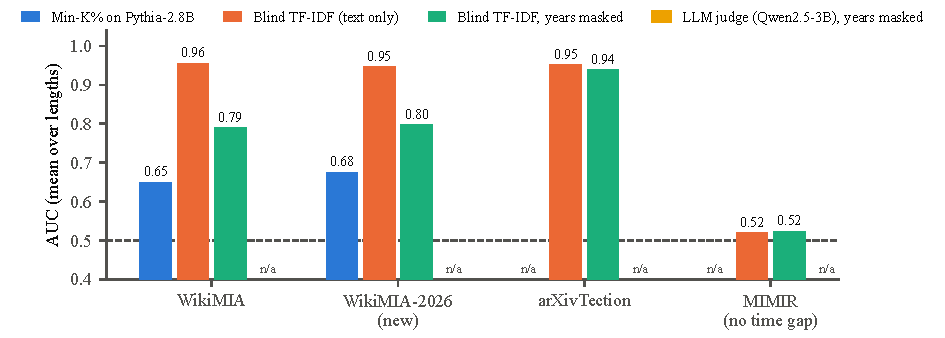
\includegraphics[width=\textwidth]{figures/benchmarks.pdf}
\caption{Min-K\% with model access (blue) against three readers without it. On the two date-defined Wikipedia benchmarks a text-only classifier separates members from non-members far better than the attack does, and still does when every year is masked, and an LLM judge (Qwen2.5-3B) reading masked text, one passage at a time, matches or beats the attack; on MIMIR, where both classes come from the same period, every reader is at chance and Min-K\% only just above it. Min-K\% is not run on arXivTection because its labels do not match Pythia's training data (Section~\ref{sec:existing}).}
\label{fig:benchmarks}
\end{figure*}

\subsection{Min-K\% transfers to WikiMIA-2026}

On WikiMIA-2026, Min-K\% with Pythia-2.8B reaches \NewMinK{} AUC (mean of the four lengths), slightly above its \RepMinK{} on the original WikiMIA, and is again the best of the five methods (PPL \NewPPL{}, Lowercase \NewLower{}, Zlib \NewZlib{}, Smaller Ref \NewRef{}). The size trend also holds (\NewSizeTrend{} for 160M, 1.4B and 2.8B; Figure~\ref{fig:size}). Taken at face value, the paper's claims generalise to a fresh benchmark built the same way. Its errors are telling, though. The non-members Min-K\% finds most member-like are templated recurring events (the 2026--27 ISU Junior Grand Prix, the 32nd Actor Awards) whose wording repeats earlier editions the model has seen; the members it finds least member-like are full of rare names (Storm Eva, ``also called Chuck, Staffan'') or were rewritten later: the page \emph{Madha Gaja Raja}, created in 2012, now describes a film released in 2025. Min-K\% measures familiar wording, which tracks membership only in part.

\subsection{But the text alone separates the classes}
\label{sec:blind}

Following \citet{das2024blind}, I trained a \emph{blind} classifier that never sees a model: TF-IDF features of word unigrams and bigrams with logistic regression, evaluated by 5-fold stratified cross-validation with the vectoriser fitted inside each training fold (\texttt{scripts/blind\_baseline.py}). On WikiMIA it reaches \BlindWikiRaw{} AUC, against \RepMinK{} for Min-K\%; on WikiMIA-2026, \BlindNewRaw{} against \NewMinK{}. No learning is needed for most of this: scoring each passage by the latest year it mentions gives \BlindWikiYear{} on both. With every year masked the classifier still reaches \BlindWikiNoyr{} and \BlindNewNoyr{}, and its most informative features show why: \emph{will} and \emph{will be} for non-members, \emph{was} for members, plus topical words such as \emph{Trump}, \emph{satellite} and \emph{Iran} for 2026. On arXivTection it reaches \BlindArxRaw{} (\BlindArxNoyr{} with years masked, led by \emph{LLMs}) with folds grouped by source paper; without grouping, excerpts of one paper land on both sides and the AUC rises to \BlindArxLeaky{}.

None of this shows Min-K\% is wrong, only that an AUC on a date-defined benchmark is likely to overstate what the attack detects about membership.

\subsection{The control: MIMIR}
\label{sec:mimirres}

On MIMIR the classes share a period, so only membership separates them. Min-K\% with Pythia-2.8B scores \MimirMinK{} (PPL \MimirPPL{}, Zlib \MimirZlib{}), with the size trend \MimirSizeTrend{} for 160M, 1.4B and 2.8B. That is 0.12--0.15 below its scores on the two date-defined benchmarks, and the per-length 95\% intervals (\MimirCI{}) reach down to chance. Model size, which adds \RepSizeGain{} AUC on WikiMIA and \NewSizeGain{} on WikiMIA-2026 between the smallest and largest model, adds \MimirSizeGain{} here, and Min-K\%'s lead over Zlib shrinks to 0.001. This agrees with \citet{duan2024membership}, who find near-chance attacks on the same data for Pythia up to 12B, trained for about one pass over a very large corpus. The blind classifier is at chance on MIMIR as well (\BlindMimirRange{}), so MIMIR is not simply harder for every method: it removes the signal that both the classifier and Min-K\% used on WikiMIA. What remains for Min-K\% is a small but consistent edge, which is what membership looks like at this scale.

\subsection{How much do the year tokens explain?}
\label{sec:masking}

Non-member passages mention recent years that Pythia has rarely seen, which are exactly the low-probability tokens Min-K\% averages. Masking every year to \texttt{YEAR} and re-running the same attack gives \MaskWikiMinK{} on WikiMIA (from \RepMinK{}) and \MaskNewMinK{} on WikiMIA-2026 (from \NewMinK{}). The year tokens alone are thus worth \MaskWikiDrop{} and \MaskNewDrop{} AUC, \MaskShareRange{} of Min-K\%'s margin over chance. Min-K\% loses more than any other attack on both benchmarks, as expected of a score built from the least likely tokens, and with years masked it is no longer the best method on either (Table~\ref{tab:results}). But masking removes only the most obvious time cue: on the same masked text the blind classifier still reaches \BlindWikiNoyr{} and \BlindNewNoyr{}, so the drop measures what the year tokens contribute, not the whole time effect.

\subsection{Min-K\% on the shift-controlled subset}
\label{sec:shiftres}

Table~\ref{tab:shift} applies the propensity controls of Section~\ref{sec:matched}. On the matched subsets the blind classifier is near chance (\ShiftBlindRange{}), yet Min-K\% keeps an AUC of \ShiftMinKRange{} (weighted mean \ShiftMinKPooled{}), close to its full-set values; stratifying on the blind score instead of matching gives the same picture. Min-K\% is therefore not simply re-detecting the cues a bag-of-words model finds. Two caveats keep this from being proof of memorisation. The subsets are small (\ShiftNMin{}--\ShiftNMax{} passages) and the intervals wide. And a name that first appears in 2026 is invisible to TF-IDF, which needs to see a word in training, but is exactly what a language model trained in 2020 finds improbable: novelty of this kind is still time, not membership. Only a benchmark without a time gap, such as MIMIR, separates the two.

\begin{table}[t]
\centering\scriptsize
\setlength{\tabcolsep}{2.6pt}
\begin{tabular}{@{}llrcccc@{}}
\toprule
& & & \multicolumn{2}{c}{\textbf{matched subset}} & \multicolumn{2}{c}{\textbf{Min-K\% AUC}} \\
\cmidrule(lr){4-5}\cmidrule(lr){6-7}
\textbf{Data} & $L$ & $n$ & blind & Min-K\% [95\% CI] & full set & stratified \\
\midrule
WikiMIA & 32 & 100 & 0.57 & 0.60 [0.49, 0.71] & 0.62 & 0.60 \\
 & 64 & 64 & 0.62 & 0.63 [0.49, 0.76] & 0.61 & 0.65 \\
 & 128 & 50 & 0.56 & 0.53 [0.36, 0.70] & 0.67 & 0.54 \\
 & 256 & 36 & 0.54 & 0.76 [0.59, 0.92] & 0.70 & 0.75 \\
\addlinespace
WikiMIA-2026 & 32 & 194 & 0.54 & 0.62 [0.54, 0.69] & 0.65 & 0.62 \\
 & 64 & 126 & 0.55 & 0.65 [0.55, 0.74] & 0.67 & 0.66 \\
 & 128 & 70 & 0.53 & 0.74 [0.62, 0.86] & 0.71 & 0.72 \\
 & 256 & 26 & 0.50 & 0.74 [0.52, 0.92] & 0.67 & 0.77 \\
\bottomrule
\end{tabular}

\caption{Shift-controlled evaluation. \emph{Matched}: members and non-members paired on the blind TF-IDF score (Section~\ref{sec:matched}); $n$ passages; the blind classifier's own AUC on the subset, then Min-K\%'s with a bootstrap 95\% CI. \emph{Stratified}: Min-K\% AUC over member/non-member pairs in the same blind-score quintile.}
\label{tab:shift}
\end{table}

\subsection{Humans and LLM judges on the same pairs}
\label{sec:judges}

\paragraph{Role of the LLM judge.} Membership is not a property of the text, so an LLM judge cannot replace the ground truth or the AUC; a judge that could tell members from non-members by reading would signal a broken benchmark. It instead automates the human audit of Section~\ref{sec:annotation}, so that every passage of every benchmark can be audited, which three people cannot do. I used two small open models from different families, Qwen2.5-3B-Instruct \citep{qwen2024qwen25} and Phi-3.5-mini-instruct \citep{abdin2024phi3} (3.1B and 3.8B parameters), in float16 on a T4 (notebook \texttt{04\_controls\_and\_judge}). Each judge receives the annotators' instructions, which act as its annotation guideline, in the two modes that evaluator models such as Prometheus~2 support \citep{kim2024prometheus}: \emph{pairwise}, with both passages as the humans saw them, and \emph{pointwise}, one passage at a time (Appendix~\ref{app:prompts}). Either way it must answer A or B. The verdict is read from the probabilities of the two answer letters, which hold \JudgeQwenMass{} and \JudgePhiMass{} of the probability mass, so no parsing is needed and every answer has a confidence. Each pair is asked twice with the passages swapped, which measures position bias, a known weakness of LLM judges \citep{zheng2023judging}, and the two probabilities are averaged to cancel it.

\paragraph{Results.} Table~\ref{tab:annotation} gives accuracy on the annotated pairs, where a correct answer picks the 2026 passage. Skimming in round 1, the humans' majority vote was at chance (\MajorityAccOne{}; individuals \HumanAccRangeOne{}, only A2 above chance), while on the same pairs the blind classifier reached \PairBlindNoyrOne{} with years masked and Min-K\% ordered \PairMinKOne{} correctly. At a glance the shift is largely invisible to people; it lives in regularities of tense and vocabulary that a classifier aggregates over many examples. Reading in full in round 2, humans reached \HumanAccRangeTwo{} (majority \MajorityAccTwo{}). Two of the three, A1 and A3, came close to Min-K\% on the same 40 pairs (\PairMinKTwo{}), though only A1's interval excludes chance; A2 was at chance, and the majority's interval still includes 0.5. Round 2 is exploratory, as the pairs had been seen before: on the same 40 pairs round 1 gave A1--A3 0.35, 0.68 and 0.47, so two improved and one fell. Read carefully, part of the shift becomes visible, but one person judging one pair is a far weaker detector than a classifier trained on a thousand passages (\PairBlindNoyrTwo{} here, years masked). My own score should be discounted, since I built the data.

The pairwise judges show position bias in its most extreme form: both answer B, whichever passage is second (mean $P(\mathrm{A})$ \JudgeQwenPA{} and \JudgePhiPA{}), so the two orders agree on \JudgeQwenConsistent{} and \JudgePhiConsistent{} of pairs, and keeping only consistent verdicts would leave at most two. Averaging the orders cancels the bias, but what is left for Qwen is a difference in the sixth decimal place, so their accuracies (\JudgeQwenPairAccOne{} and \JudgePhiPairAccOne{} on the 100 pairs) carry little weight. The residual is not pure noise: Cohen's $\kappa$ with the round-2 human majority is \KappaQwenMajorityTwo{} (Qwen) and \KappaPhiMajorityTwo{} (Phi), and \KappaJudgesTwo{} between the judges, all above the humans' agreement with each other. By the usual test of a judge, agreement with people against agreement among people, both judges match a human here, but only because the humans agree so little. The pointwise format has no position to prefer, and there the judges work. Over every passage one at a time, with every year masked and no access to Pythia, their AUC is \JudgeQwenWiki{} (Qwen) and \JudgePhiWiki{} (Phi) on WikiMIA, above Min-K\% with Pythia-2.8B (\RepMinK{}); \JudgeQwenNew{} and \JudgePhiNew{} on WikiMIA-2026, close to it (\NewMinK{}); and \JudgeQwenMimir{} and \JudgePhiMimir{} on MIMIR, chance. Their higher WikiMIA score may partly reflect knowledge of its 2023 events, which their training data can include; 2026 events they cannot know. As an audit the judge works: untrained on the labels, it flags both date-defined benchmarks as separable by era and passes MIMIR.

\begin{table*}[t]
\centering\footnotesize
\begin{tabular}{@{}lcccc@{}}
\toprule
& \multicolumn{2}{c}{\textbf{Round 1}: 100 pairs, no time limit} & \multicolumn{2}{c}{\textbf{Round 2}: 40 pairs, buttons locked 10\,s} \\
\cmidrule(lr){2-3}\cmidrule(lr){4-5}
\textbf{Reader} & median s/pair & accuracy [95\% CI] & median s/pair & accuracy [95\% CI] \\
\midrule
A1 (author) & 4.1 & 0.47 [0.38, 0.57] & 21.1 & 0.68 [0.52, 0.80] \\
A2 & 1.9 & 0.64 [0.54, 0.73] & 12.9 & 0.47 [0.33, 0.63] \\
A3 & 1.5 & 0.51 [0.41, 0.61] & 16.5 & 0.65 [0.50, 0.78] \\
Human majority vote &  & 0.54 [0.44, 0.63] &  & 0.62 [0.47, 0.76] \\
\midrule
LLM judge: Qwen2.5-3B &  & 0.53 [0.43, 0.62] &  & 0.50 [0.35, 0.65] \\
LLM judge: Phi-3.5-mini &  & 0.64 [0.54, 0.73] &  & 0.65 [0.50, 0.78] \\
Min-K\% (Pythia-2.8B) &  & 0.64 [0.54, 0.73] &  & 0.68 [0.52, 0.80] \\
Blind TF-IDF (raw text) &  & 0.97 [0.92, 0.99] &  & 0.95 [0.83, 0.99] \\
Blind TF-IDF (years masked) &  & 0.83 [0.74, 0.89] &  & 0.80 [0.65, 0.90] \\
\midrule
Fleiss' $\kappa$, 3 humans & \multicolumn{2}{c}{0.005} & \multicolumn{2}{c}{0.100} \\
\bottomrule
\end{tabular}

\caption{Recency judgements on the annotated WikiMIA-2026 pairs (64 words, years masked); a correct answer identifies the 2026 passage, and accuracy over member/non-member pairs estimates AUC. Round 2's 40 pairs are a subset of round 1's 100. A1 is the author. Accuracy excludes ``can't tell''; Wilson 95\% intervals. Machine rows score the same pairs.}
\label{tab:annotation}
\end{table*}

\subsection{How the new results relate to the replication}

The replication and the new data agree on the paper's \emph{measurements}: on two date-defined benchmarks built three years apart, Min-K\% beats the other attacks by a similar margin and improves with model size. They disagree on the \emph{interpretation}: on both, a text-only classifier does far better than the attack and LLM judges about as well, and when the time gap is removed, on MIMIR, the attack falls to \MimirMinK{} while the blind classifier and both judges fall to chance with it. The paper's numbers reproduce; the evidence that they measure pretraining-data membership rather than time is, at the scale tested here, weak.

% =====================================================================
\section{Ethical Considerations}
\label{sec:ethics}

\paragraph{In the original paper.} The paper has no ethics statement or limitations section, although ICLR encourages one; its ethical framing is the motivation in its introduction (copyrighted text, personal data and test sets inside training corpora). Membership inference is a privacy attack: a reliable detector can reveal that a person's text, such as an email, medical note or forum post, was in a model's training set. The paper frames its use as defensive (copyright, contamination, unlearning audits), but the same tool serves an adversary. My results sharpen a further issue: the copyright study sets its threshold on BookMIA, a date split of the kind Section~\ref{sec:results} questions, then lists by title the 20 Books3 books it finds most likely to be in GPT-3's training data. Authors and developers may act on such claims, which need a validity check that a date split cannot give. WikiMIA is released under MIT, while its passages are Wikipedia text licensed CC BY-SA 4.0 \citep{wikipediacopyright}, which requires attribution and share-alike; records carry no title or page identifier, so attribution cannot be recovered from the dataset. A paper about detecting unlicensed use of text should model licence compliance in its own data.

\paragraph{Publishing on the new data.} In the terms used to analyse ACL ethics sections \citep{benotti2022ethics,karamolegkou2025ethical}, the expected benefit here is better-calibrated claims about what training-data detectors show; the potential harms fall mainly on people named in the data and on annotators; and the most vulnerable group is victims named in event pages, discussed below. Under the \emph{Australian Code for the Responsible Conduct of Research} \citep{acrcr2018}, the principles most at stake are \emph{honesty} and \emph{transparency} in reporting and \emph{fairness} in the use of others' work. I report results that weaken the paper's interpretation alongside those that support it, give confidence intervals rather than single numbers, release every script, log and per-passage score, and record the bug fixed in the dataset build rather than hiding it. Credit goes to the original authors, the data creators and Wikipedia's editors. WikiMIA-2026 is released under CC BY-SA 4.0 with each passage's title and revision id, so attribution and the exact text are recoverable. MIMIR's access terms are respected: the files are kept out of the public repository and results store only indices and hashes. Each model was used under its published licence.

Wikipedia event pages name real people. Seventeen WikiMIA-2026 pages (about 1.5\%) are about the killing, murder or kidnapping of a named person, often a private individual; one concerns a five-year-old Aboriginal Australian girl, whose page already uses a cultural substitute name, and protocols around naming deceased Aboriginal and Torres Strait Islander people apply. The text is already public, but republishing it in a research dataset concentrates it, so for publication I would exclude these pages, honour removal requests, and keep them out of figures, as I did in Figure~\ref{fig:snippets}. I found these pages only after the annotation task was sent: five of the 100 pairs describe killings, including that child's, and round-1 annotators were not warned. Round 2 left those pairs out and added a content note to the instructions; any repeat should screen items before they are sent.

The annotation is human research under the \emph{National Statement} \citep{nationalstatement2025}. Its risk is low, no more than the inconvenience of about 20 minutes of reading per round: participation was voluntary and unpaid, consent was recorded on the page, only initials were collected, annotators could stop at any time, and released files replace initials with A1--A3. For a class project I did not seek formal review; for a publication the study would need low-risk ethics review before any data were collected, and my two volunteers being acquaintances creates a mild pressure to agree that a review would consider. Membership inference itself is dual use, but this project adds no attack capability. Like other work on attacks \citep{li2024seeing}, it discloses a weakness so that others can take it into account; here the weakness is that benchmark AUCs overstate what attacks detect, which mainly helps those assessing claims about models. Compute was a few T4 GPU-hours.
% =====================================================================
\section{Conclusions and Reflections}
\label{sec:conclusion}

\paragraph{Replication.} The paper replicates. With the authors' unmodified code and current libraries, Min-K\% on WikiMIA with Pythia-2.8B scores \RepMinK{} against the published 0.67, all five methods are within about 0.02, and the size and length trends hold. Getting there required finding six traps in the code. The paper's ranking of Min-K\% over Zlib is within sampling noise at Pythia scale.

\paragraph{Generalisation.} The method transfers to a benchmark built the same way three years later, and that is the problem: both benchmarks are separable without any model at AUC 0.95. Where the period is held fixed, on MIMIR, Min-K\% scores \MimirMinK{}, its size trend shrinks from \RepSizeGain{} to \MimirSizeGain{}, and it ties Zlib; masking years removes only \MaskShareRange{} of its WikiMIA margin; and small LLM judges with no access to Pythia come within 0.04 of it or beat it on both date-defined benchmarks. The shift-controlled subset suggests some signal beyond bag-of-words cues, but it is small, and that signal may still be novelty rather than membership.

\paragraph{Reflections.} Building WikiMIA-2026 with matched categories did not remove the confound: time leaks through the language of a text, not only its topic, so a date-defined benchmark is confounded by design, and membership is better defined from a known corpus, as in MIMIR. Reading the data mattered as much as running the code: the redirect bug, the page-split label noise and the passages about named victims were all found by reading examples. Annotation was harder than expected, and my first design let it fail: with 100 pairs and no minimum reading time, all three of us skimmed and agreed no better than chance. A one-person pilot would have caught this; round 2's reading lock is the fix, and hidden gold questions, the unit's check on crowd workers, would be the next. Likewise, ten judge pairs run in both orders first would have exposed the position bias; pointwise judging should have been the main design.

\bibliography{refs}

\appendix

\section{Six traps in the original code}
\label{app:traps}

(1)~There is no \texttt{requirements.txt}; versions had to be chosen and recorded. (2)~\texttt{run.py} imports \texttt{openai} unconditionally, and its GPT-3 path calls \texttt{text-davinci-003}, retired in January 2024, so the paper's GPT-3 rows cannot be reproduced at all. (3)~\texttt{run.py} stores the \emph{negated} Min-K\% mean and \texttt{eval.py} negates again inside \texttt{roc\_curve}; a reimplementation that misses one sign inverts the ROC curve. (4)~The repository ships an \texttt{out/} directory with the authors' own LLaMA-13B results, which any script that globs for \texttt{auc.txt} picks up instead of one's own. (5)~\texttt{eval.py} labels its third number ``TPR@0.1\%FPR'' but computes TPR at 5\% FPR. (6)~\texttt{eval.load\_jsonl} silently shuffles rows with a fixed seed: AUC is unaffected, but per-passage outputs no longer line up with the input file, so every later join in this project uses the passage text or its hash, never the row number.

\section{LLM-judge prompts}
\label{app:prompts}

Both judges receive one user message through their own chat template, with no system message other than the template default.

\noindent\textbf{Pairwise} (\texttt{\{a\}}, \texttt{\{b\}} are the masked passages): \emph{Below are two passages, each from the start of a Wikipedia article. Every year has been replaced with the word YEAR. One passage describes an older event and the other describes a newer event. Clues people use: names of politicians or office holders, technology, how many times an event has already happened (``the 61st edition''), whether the text says something will happen, and so on. Passage A: """\{a\}""" Passage B: """\{b\}""" Which passage describes the more recent event? Answer with a single letter: A or B.}

\noindent\textbf{Pointwise}: \emph{Below is a passage from the start of a Wikipedia article. Every year has been replaced with the word YEAR. [same clues] Passage: """\{text\}""" Is the event or topic of this article from before 2017, or from 2023 or later? A) before 2017 B) 2023 or later. Answer with a single letter: A or B.}

\end{document}
